\title{\textbf{Automatic Projector Tilt Compensation System}}
\author{Ganesh Ajjanagadde \quad James Thomas \quad Shantanu Jain}
\date{\today}
\documentclass{article}

\usepackage{graphicx} % for including images
\usepackage{float} % for floating figures, i.e can place/modify images in fancy ways

%Please place images in img/ subdir of proj_proposal for clean directory structure

\begin{document}
\maketitle

%\begin{abstract}
%Our goal is to design a system that corrects the input to a projector if it is tilted so that its output appears unskewed.
%We will be projecting the display of a PC, and will connect the computer's VGA output to the FPGA board, and the FPGA board's VGA output to the projector.
%We will mount an accelerometer on the projector and measure its signals to determine the projector's tilt angles on two axes.
%We will run algorithms on the FPGA that correct the VGA input based on the tilt angles and produce the results at the VGA output for the projector to display.
%Finally, we will design digital logic that produces a voice specifying the new tilt angles whenever they are changed.
%The project was motivated by the increasing prevalance of portable projectors that benefit from fast automated setup.
%\end{abstract}

\section{Introduction}
Due to the advances in semiconductor technology, today's display projectors can incorporate fairly sophisticated digital processing algorithms for various enhancements to the visual appearance.
Moreover, there is an increasing prevalence of portable projectors that benefit from fast, automated setup.
One desired functionality is keystone/tilt correction.
This means that even when the projector is tilted, the projector is able to ``pre-warp'' the image so that its output appears unskewed.

In this project, we will be projecting the output of a camera, and will connect the camera's output to the FPGA board, and the FPGA board's VGA output to the projector.
We will mount an accelerometer on the projector and measure its signals to determine the projector's tilt angles on two axes.
We will run algorithms on the FPGA that correct the camera output based on the tilt angles and produce the results at the VGA output for the projector to display.
We will calibrate the accelerometer through a special calibration mode.
As a stretch goal, we will also attempt to use the camera combined with the accelerometer itself to calibrate by projecting a known image, such as a white rectangle.
This should result in a gain to the quality of keystone/tilt correction, and one of our goals is to qualitatively observe and quantify such differences in quality.
Finally, we will design digital logic that produces a voice with help commands, and also lets the user know of the new tilt angles whenever they are changed.

\section{Implementation}

\subsection{Modules and Dataflow in Our Projector Tilt Compensation System}
\begin{figure}
\centering
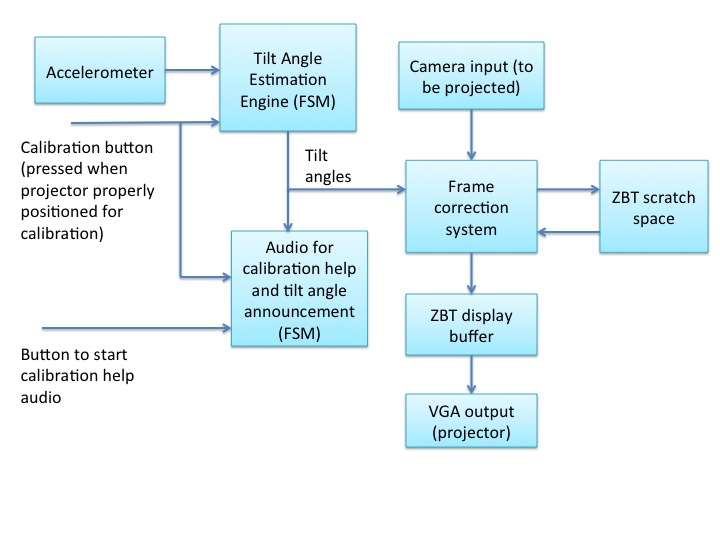
\includegraphics[width=\textwidth]{img/block_diag}
\caption{An overview of the modules in our system. An accelerometer will feed acceleration data for the two dimensions of interest into an engine that estimates the actual tilt angles for these two dimensions. These angles will be sent as input to a module that accordingly pre-warps the camera input and sends it to the VGA output to be projected. We will have a calibration system that will instruct the user with audio to position the projector so that its output is rectangular and then hit a calibration button, giving the tilt angle estimation engine some reference points. The audio system will also announce the tilt angles when they change. There will also be some switches that allow the user to manually adjust the quadrilateral into which the camera input is pre-warped, which will help us during development in determining the warping required for different tilt angles. Some of the most challenging parts of this system include reading sufficiently granular data from the accelerometer, properly converting from accelerometer data to tilt angles and warping quadrilaterals, and pipelining and optimizing the algorithms for warping the camera input so that they can run in real time.}
\end{figure}

\subsection{Modules}

\subsubsection{Accelerometer}
The accelerometer is an Analog Devices 3 axis accelerometer ADXL362.
The ADXL362 gives acceleration values at an 8 bit resolution, and is controlled via a SPI interface.
Thus, this module will implement the appropriate SPI interface so as to make the raw data available to the FPGA.
Unfortunately, this data is extremely noisy.
As such, this module will also implement a low-pass filter in order to suppress this noise.
For simplicity, we will use a moving average filter.

\subsubsection{Tilt Angle Estimation Engine}
The tilt estimation engine will accept a calibration input (e.g a button) in order to normalize the accelerometer readings based on the values for zero tilt.
Basically, it subtracts off the readings for a neutral position in order to get a consistent value for the tilt reading.

\subsubsection{Audio}
The audio module will read audio from the stored compact flash and will play the appropriate audio depending on the input signal to the module.
For instance, when the user requests help regarding calibration via pressing the appropriate button,
it goes into a state in which it does a looping playback instructing the user how to adjust the projector so that the output appears unskewed.
When a change in tilt is detected,
the percentage of pixels lost due to the ``pre-warping'' will change and the audio enine will play a recording specifying the new percentage.
Other audio will be added/updated as needed as our user interface changes.

\subsubsection{Frame correction system}
The frame correction system will be responsible for ``pre-warping'' the image based on the current accelerometer readings from the tilt estimation engine.
The camera output is stored in a ZBT buffer, and is updated on every NTSC clock cycle.
The ``pre-warping'' transformation (mathematically a perspective transform) is computed in a ZBT scratch buffer.
The output frame from the ``pre-warping'' is stored in a ZBT display buffer.
An auxiliary module will then feed the pixels in the display buffer to the VGA output at the appropriate vsync clock edge.

\section{Timeline}
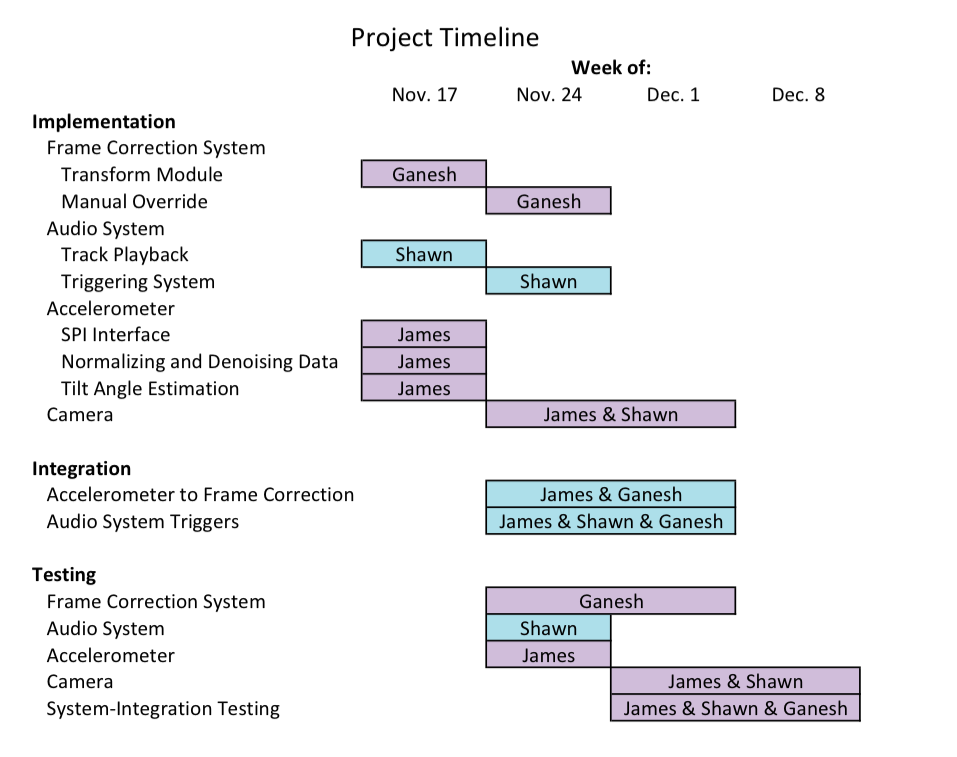
\includegraphics[width=\textwidth]{img/Timeline}
There is five weeks time in which to complete the project. In these five weeks, we envision four major stages to the project:
\begin{enumerate}
	\item Initial Implementation and Unit Testing \hfill \\
		Time: 2 weeks \hfill \\
		In this stage, each team member will create an initial implementation of modules he is responsible for. He is expected to have his modules working as a standalone component. Each module will include simple test benches to confirm the module's standalone functionality. Following the unit testing style will reduce bugs during the module integration stage. Ganesh will focus on the ``Frame Correction System'', working to create an implementation of his algorithm. Shantanu will focus on the ``Audio System'', implementing the playback system for a set of audio tracks. He will be challenged in testing the system's ability to switch between a set of non-predetermined audio tracks based on arbitrary triggers. James will focus on the ``Accelerometer''. Because he is dealing with an external component, he will face challenges of how to interpret the data coming from the accelerometer. He may have to compensate for non-linear data from the device, and adjust his module's implementation to compensate. He will be challenged by having to test some of his code by physically manipulating the accelerometer by hand, instead of entirely automatically by test benches. 
	\item Module Integration; System Building \hfill \\
		Time: 2 weeks \hfill \\
		This stage will connect the individual modules from the implementation stage together to form the initial system. This is expected to be the most hands-on and collaborative stage, as mistakes will often have a domino effect on the system. In the worst case, we may have to modify parts of our system design or change the behavior of some modules in order to compensate; in lesser situations, bugs may be uncovered and fixed. This is expected to be the lengthiest stage.
	\item System-Integration Testing \hfill \\
		Time: 1 week \hfill \\
		After the system has been put together and functions minimally, the team will focus on system-integration testing. The goal of testing is to make the system robust. In this stage of testing, all three team members will be involved in testing the system holistically. Testing will reflect the user workflows comprehensively - all the routes through the system will be tested. Because of this requirement, this stage of testing will require knowledge about the implementation of all the modules, requiring all members to be involved. The team may recruit additional testers to check for the user-friendliness of the systemas well. These test subjects will be other students in the lab and friends of the team members. 
	\item Stretch Goals \hfill \\
		Time: As available \hfill \\
		Once the system satisfies the test coverage plan, the team will focus on adding additional features to the system, as constrained by time. These possible additional features are described below.

\end{enumerate}

\section{Individual Responsibility}
\begin{description}
	\item{Ganesh}
	\begin{itemize}
		\item Algorithm - Identifying the appropriate algorithm, considering factors of complexity, hardware constraints, and implementability.
		\item Transform Module - Implementing the algorithm, with input parameters
	\end{itemize}
	\item{James}
	\begin{itemize}
		\item Accelerometer - Identifying the appropriate type and model, interfacing with the labkit.
		\item Calibration module - Entering calibration mode, collecting data, making it available as necessary.
		\item Test Setup - attaching accelerometer to projector, wiring to labkit.
		\item Camera - Receiving the data from the camera and displaying it on the projector. Will lead the development of this module and will collaborate with Shantanu. 
	\end{itemize}
	\item{Shantanu}
	\begin{itemize}
		\item Audio output - Identifying necessary audio outputs, triggers for audio. Recording audio, transforming it into the appropriate format.
		\item Audio module - loading audio onto the labkit, standardizing trigger parameters.
	\end{itemize}
\end{description}

\section{Stretch Goals}
	\begin{itemize}
		\item Camera-based adjustment \hfill \\
			The camera-based adjustment would augment the accelerometer by displaying a test pattern output to the projector and using an edge detection/corner detection algorithm to determine the skew caused by the projector's tilt. It would be able to correct the projector image in a wider variety of scenarios, including variable distance to the screen. This is difficult as it is complex and time consuming to interface the camera with the labkit and implement these additional algorithms.
		\item External display of transformed image\hfill \\
			View the transformed image on a non-distorted screen, such as a PC LCD monitor.
	\end{itemize}

\section{Conclusion}
In summary, we aim to build a system that can pre-warp the input to a tilted projector so that the projected output appears properly rectangular. We will use an accelerometer to determine the angles of tilt of the projector in two dimensions, and have logic on an FPGA that warps camera input in real time and sends it to the projector. We will have a comprehensive audio system that provides calibration assistance and reads out statistics on the perspective transform to the user. Our system is practically valuable due to the increasing prevalence of portable projectors that are hard to perfectly align on surfaces.
\end{document}
